\section{Methodology}

\subsection{Performance Metrics}

To determine if using computer vision is an adequate method to estimate 
emissionscoefficients in New York City, the vehicle detection pipeline must be 
rigorously evaluated. Unlike standard image classification, object detection 
requires assessing two distinct tasks simultaneously: accurately localizing a 
vehicle within a complex urban environment and correctly classifying its 
emissions profile category (e.g., distinguishing a heavy-duty vehicle from a 
light-duty vehicle). This subsection details the metrics selected to quantify 
the model's performance. It begins by establishing the spatial evaluation 
criteria, builds toward aggregate threshold-agnostic metrics like mean Average 
Precision (mAP), and concludes by justifying these choices against traditional 
classification metrics that fall short in dynamic spatial contexts.

\subsubsection{Intersection over Union}

Before assessing the classification accuracy of the model, it is necessary to 
quantify the spatial accuracy of the predicted bounding boxes. This is achieved 
using the Intersection over Union (IoU) metric. IoU measures the overlap between 
a predicted bounding box and a ground truth bounding box. It is calculated as 
the area of their intersection divided by the area of their union.

\begin{figure}[!htbp]
    \centering
    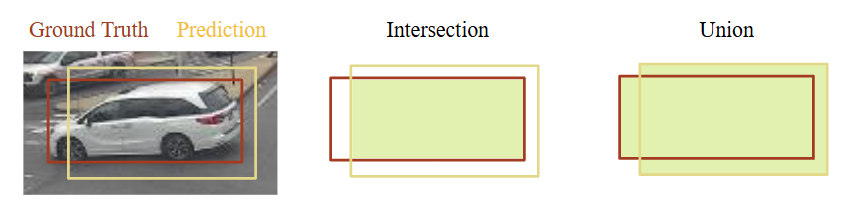
\includegraphics[height=3.5cm]{figures/methodology/4_2_intersection_union.png}
    % \caption{Confusion Matrix}
    % \label{fig:conf_matrix}
\end{figure}

\begin{figure}[!htbp]
    \centering
    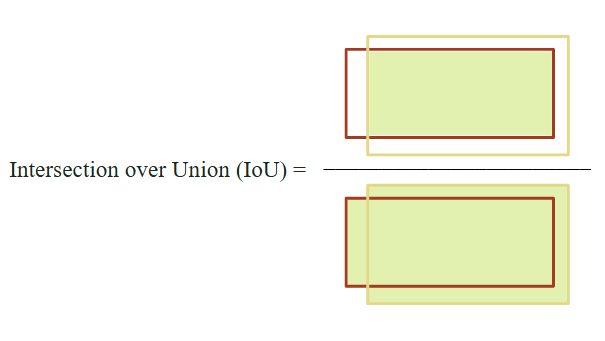
\includegraphics[width=0.6\textwidth]{figures/methodology/4_2_iou_calculation.png}
    \caption{IoU Calculation}
    \label{fig:iou_calc}
\end{figure}

An IoU score ranges from 0 (no overlap) to 1 (perfect alignment). By
establishing an IoU threshold (ex., 0.50), we define the strictness required 
for a spatial prediction to be considered valid.

\subsubsection{Confusion Matrix}

\begin{figure}[!htbp]
    \centering
    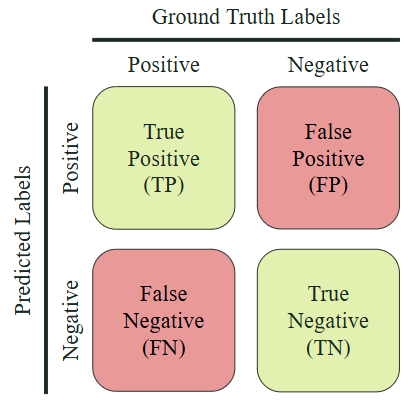
\includegraphics[height=6.5cm]{figures/methodology/4_2_confusion_matrix.png}
    \caption{Confusion Matrix}
    \label{fig:conf_matrix}
\end{figure}

With a defined IoU threshold, the traditional elements of a confusion matrix 
(Figure~\ref{fig:conf_matrix})
can be adapted for object detection. Unlike pure image classification, where every 
image has a discrete label, object detection occurs in a continuous spatial 
domain. This is because bounding box coordinates can take on virtually infinite 
combinations across an image, so a model's spatial prediction will rarely align 
pixel-for-pixel with a human annotation. Thus, setting a threshold on the IoU 
metric acts as a spatial tolerance mechanism, converting continuous coordinate 
overlaps into the discrete \textit{True Positive} or \textit{False Positive} 
categories required to calculate performance metrics. Within the context of this
project, the entries of the confusion matrix correspond to: 

\begin{itemize}
    \item \textbf{True Positive (TP)}: A detection that matches a human-annotated
    ground truth box of the correct vehicle class with an IoU $\geq$ the defined 
    threshold. For example, the model successfully draws a bounding box around a 
    sedan and correctly classifies it as a Light-Duty Vehicle (LDV) with an IoU 
    that exceeds the threshold.

    \item \textbf{False Positive (FP)}: A predicted box that fails either the 
    spatial or classification criteria. In the context of urban traffic 
    monitoring, this typically occurs in three ways:
    \begin{enumerate}
        \item{\textit{Misclassification}}: The model perfectly localizes an LDV but
        incorrectly classifies it as a Heavy-Duty-Vehicle (HDV), skewing the 
        emissions profile for that frame.

        \item{\textit{Poor Localization}}: The model correctly identifies a Bus, but the
        bounding box only captures a fraction of the vehicle, resulting in an 
        IoU below the required threshold.

        \item{\textit{Background/Duplicate}}: The model hallucinates a vehicle where 
        there is only an empty patch of road, or it draws two separate bounding 
        boxes over the same motorcycle.
    \end{enumerate}

    \item \textbf{False Negative (FN)}: A ground truth vehicle that the model 
    failed to detect entirely, or localized so poorly that it was discarded. 
    For instance, an LDV partially occluded by a building is completely ignored 
    by the model, resulting in an uncounted emissions source.

    \item \textbf{True Negative (TN)}: Conceptually, a true negative represents
    every possible empty region in an image (such as patches of bare asphalt, 
    sidewalks, buildings, or sky) where the model correctly predicted that \textit{no} 
    vehicle was present. Because the number of empty background regions in a 
    dense urban scene is effectively infinite, True Negatives mathematically 
    distort traditional evaluation metrics and are therefore excluded from 
    object detection performance calculations.
\end{itemize}

\subsubsection{Precision-Recall Curve}
Using the \textit{TP}, \textit{FP}, and \textit{FN} counts defined above, we can calculate Precision and 
Recall to evaluate the pipeline's ability and reliability in tracking 
urban traffic.

\begin{itemize}
    \item \textbf{Precision} measures the reliability of the model’s vehicle predictions.

    \begin{equation}
    Precision = \frac{TP}{TP + FP}
    \end{equation}

    In the context of this project, out of all the bounding boxes the model predicted 
    for a certain class (ex. Claiming to detect 50 HDVs), what fraction were correct? 
    A high precision score ensures the model is not predicting false ``ghost'' 
    vehicles or misclassifying vehicle types.

    \item \textbf{Recall} measures the model's ability to find vehicles in the frame.

    \begin{equation}
    Recall = \frac{TP}{TP + FN}
    \end{equation}

    Recall indicates out of all the actual ground truth objects present, what 
    fraction did the model successfully detect? A high recall score ensures 
    emission sources are not undercounted in the final analysis.
\end{itemize}

Modern object detectors like the DETR output a confidence score with each 
predicted bounding box, creating a trade-off between Precision and 
Recall. Lowering the confidence threshold allows the model to predict more 
vehicles (increasing Recall), but it simultaneously increases the risk of 
capturing background noise as valid vehicles (False Positives), thereby 
lowering Precision. By calculating Precision and Recall at every possible 
confidence threshold and plotting the results, we generate the Precision-Recall 
(PR) Curve.

(insert average looking PR curve)
